\documentclass[12pt, a4paper]{article}
\usepackage[UTF8, fontset=fandol]{ctex}
\usepackage{sectsty}
\usepackage{url}
\usepackage{geometry}
\usepackage{amsmath, amssymb}
\usepackage{graphicx}
\usepackage{booktabs}
\usepackage{hyperref}
\usepackage{cite}
\usepackage{setspace}
\usepackage{listings}
\usepackage{xcolor}
\usepackage{pgffor}
\usepackage{float}
\usepackage{pgfmath}
\usepackage{caption} % 在导言区添加
% 设置页面边距
\geometry{a4paper, top=2.5cm, bottom=2.5cm, left=2.5cm, right=2.5cm}

% 设置行间距
\onehalfspacing

% 设置超链接样式
\hypersetup{
    colorlinks=true,
    linkcolor=black,
    urlcolor=blue,
    citecolor=black
}

% 设置代码块样式
\lstset{
     basicstyle=\ttfamily\small,
     keywordstyle=\color{blue},
     commentstyle=\color{gray},
     stringstyle=\color{red},
     breaklines=true,
     numbers=left,
     numberstyle=\tiny,
     frame=single,
     language=Python % 可根据需要更换为 C, C++, Java 等
   }


\title{GAN系列模型实验报告}
\author{高家璇 3023244275}
\begin{document}



\maketitle
\begin{center}
    \includegraphics[width=0.8\textwidth]{/Users/slkgaw/Proj/GANS/visual/BigGAN/512x512_random/random_samples_512_004.jpg}
\end{center}
\begin{center}
\section*{摘要}
\end{center}

在 AIGC 如此火爆的今天,了解生成模型的鼻祖 GAN (arXiv:1406.2661)是很有必要的。
GAN 是深度学习花书的作者 Ian Goodfellow 在 2014年的一篇工作,引发了一股 GAN 生模型的浪潮,
这股生成模型的浪潮一直持续到现在的 Diffusion 系列。

如今 GPT 如此发达,大部分报告内容都可以由 AI 生成。
所以本报告不会花特别多的篇幅来介绍模型的理论架构或者是其他死板的内容。为了实现本实验的终极目的:帮助学生加深对 GAN 模型的架构和训练的理解。
\textbf{因此此报告将花费大规模篇幅来重点讨论 GAN 系列模型在给定下游任务时的【训练细节与训练技巧】。}

本实验实现了:
1、GAN 在 MNIST 数据集上的训练和推理。
2、在不同数据集上训练了多个数亿参数规模的 CGAN。
3、200+ 小时训练时长,60+ 训练日志文件,1000+ 样本和损失可视化。


本报告探讨了:
1、学习率调度、正则化、模型保存与加载、损失日志与阶段可视化等实用的训练技巧
2、模型训练中的张量数据并行、分布式与混合精度训练策略
3、模型训练中的数据增强与预处理技巧,以及超参数分析
4、GAN 在建模复杂数据分布时的模式坍塌问题



本实验全部代码和构建记录:\url{https://github.com/slkhms777/GANS}

生成模型综述与主流模型代码:\url{https://github.com/slkhms777/AIGC}



% 正文
\newpage
\begin{center}
\section*{引言}
\end{center}

生成对抗网络(Generative Adversarial Networks, GANs)自 2014 年由 Goodfellow 等人提出以来,已成为深度学习领域最具影响力的创新之一。GAN 通过生成器与判别器的对抗性训练,使生成器能够逐步提升生成样本的质量,最终达到以假乱真的效果。

然而,原始 GAN 在实际应用中常常面临训练不稳定、模式坍塌(mode collapse)、梯度消失等问题。为了解决这些挑战,研究者们提出了多种改进模型,其中较为典型的包括 Wasserstein GAN(WGAN)和条件生成对抗网络(Conditional GAN, CGAN)。

\textbf{WGAN(Wasserstein GAN)} 针对训练不稳定和模式坍塌问题进行了有效改进。其核心思想是采用 Wasserstein 距离(又称 Earth Mover 距离)来衡量真实分布与生成分布之间的差异,替代了原始 GAN 中的 JS 散度。WGAN 的主要特点包括:

1. 以 Wasserstein 距离为损失函数,提升训练稳定性;

2. 判别器(Critic)输出实数值而非概率;

3. 通过权重裁剪(weight clipping)满足 Lipschitz 连续性约束;

4. 损失函数与生成样本质量正相关,便于训练过程监控。

在此基础上,\textbf{WGAN-GP(WGAN with Gradient Penalty)} 进一步用梯度惩罚(gradient penalty)替代权重裁剪,带来了更好的 Lipschitz 约束,避免了梯度消失或爆炸等问题,使训练更加稳定,生成质量进一步提升。

\textbf{CGAN(Conditional GAN)} 则在 GAN 框架中引入了条件信息,使得生成过程可控。与原始 GAN 的无条件生成不同,CGAN 能够根据输入的类别标签等条件生成特定类型的样本。其核心思想包括:

1. 生成器和判别器均以条件信息 $c$ 作为输入;

2. 生成器 $G(z, c)$ 以噪声 $z$ 和条件 $c$ 生成样本;

3. 判别器 $D(x, c)$ 判断样本 $x$ 在条件 $c$ 下的真实性;

4. 支持按需生成特定类别样本,提升生成多样性和训练稳定性。

\textbf{BigGAN} 是 Google 于 2018 年提出的大规模高分辨率图像生成模型,在 ImageNet 等数据集上取得了突破性成果。BigGAN 通过扩大模型规模、引入自注意力机制(Self-Attention)、谱归一化(Spectral Normalization)、类别条件 BatchNorm 以及截断技巧(Truncation Trick)等方法,极大提升了生成图像的质量和多样性。其主要创新点包括:

1. 大规模训练(更大的 batch size 和更深的网络结构);

2. 在生成器和判别器中引入 Self-Attention 机制;

3. 谱归一化稳定训练过程;

4. 类别条件 BatchNorm 增强类别信息利用;

5. 截断技巧提升推理阶段生成质量。

BigGAN 的成功验证了“规模即力量”的理念,为后续如 StyleGAN、DALL-E 等更大规模生成模型的发展奠定了基础。

本实验以 MNIST、Animal-Faces 及 ImageNet-1k 等数据集为基础,重点探讨了上述模型的训练技巧及生成结果的可解释性分析。
% 目录页
\newpage
\tableofcontents

\newpage
\section{任务一,二:GAN,WGAN,CGAN 在 MNIST 上的训练以及推理}
\subsection{实验设置与方法}
\subsubsection{实验设置}
\begin{itemize}
    \item 模型架构:简单的MLP网络作为生成器和判别器
    \item 数据集:MNIST 手写数字数据集
    \item 硬件:2张 NVIDIA RTX 3090 GPU 
\end{itemize}

\subsubsection{实验方法}
在mnist数据集上,训练GAN,WGAN。通过随机采样噪声向量生成手写数字图像。
CGAN略有不同,CGAN支持类别收入,因此可以指定生成特定类别的手写数字。

\subsubsection{代码示例(仅给出GAN的代码示例)}

\begin{lstlisting}[language=Python, caption=GAN 训练主循环示例]
class Generator(nn.Module):
    def __init__(self, img_size, noise_size, num_hiddens, out_channels=1):
        super().__init__()
        self.img_size = img_size
        self.out_channels = out_channels
        self.fc1 = nn.Linear(noise_size, num_hiddens)
        self.bn1 = nn.BatchNorm1d(num_hiddens)
        self.fc2 = nn.Linear(num_hiddens, num_hiddens)
        self.bn2 = nn.BatchNorm1d(num_hiddens)
        self.fc3 = nn.Linear(num_hiddens, img_size * img_size * out_channels)
        self.relu = nn.LeakyReLU()
        self.tanh = nn.Tanh()

    def forward(self, noise):
        x = self.relu(self.bn1(self.fc1(noise)))
        x = self.relu(self.bn2(self.fc2(x)))
        x = self.tanh(self.fc3(x))
        x = x.view(-1, self.out_channels, self.img_size, self.img_size)
        return x

class Discriminator(nn.Module):
    def __init__(self, img_size, num_hiddens, in_channels=1):
        super().__init__()
        self.flt = nn.Flatten()
        self.fc1 = nn.Linear(img_size * img_size * in_channels, num_hiddens)
        self.dropout1 = nn.Dropout(0.3)
        self.fc2 = nn.Linear(num_hiddens, num_hiddens)
        self.dropout2 = nn.Dropout(0.3)
        self.fc3 = nn.Linear(num_hiddens, 1)
        self.relu = nn.LeakyReLU()
    def forward(self, image):
        x = self.flt(image)
        x = self.relu(self.fc1(x))
        x = self.dropout1(x)
        x = self.relu(self.fc2(x))
        x = self.dropout2(x)
        x = self.fc3(x)
        return x

for epoch in range(num_epochs):
    for real_imgs, _ in dataloader:
        # 判别器训练
        生成噪声 noise
        用生成器生成假图像 fake_imgs = Generator(noise)
        判别器判别真实图片 outputs_real = Discriminator(real_imgs)
        判别器判别假图片 outputs_fake = Discriminator(fake_imgs.detach())
        计算判别器损失 loss_d = criterion(outputs_real, 1) + criterion(outputs_fake, 0)
        判别器反向传播和优化

        # 生成器训练
        生成新的噪声 noise
        用生成器生成假图像 fake_imgs = Generator(noise)
        判别器判别假图片 outputs = Discriminator(fake_imgs)
        计算生成器损失 loss_g = criterion(outputs, 1)
        生成器反向传播和优化

    记录并打印每个epoch的损失,定期保存模型权重,定期生成样本图片
\end{lstlisting}

\subsection{训练细节与训练技巧}
\subsubsection{正则化}
在一般的深度学习过程中,正则化是一个非常重要的环节,因为如果确实有效的正则化,模型很容易过拟合到数据集上,导致
模型的泛化性大大降低。常见的正则化有dropout和weight decay,二者虽然实现方式不同,但本质上都是防止部分神经元
在整个模型中dominate。对于weight decay,采用限制一部分神经元的权重大小的方式来防止过拟合。而dropout则直接
丢弃部分神经元来防止过拟合,二者在原理上有异曲同工。

但是针对任务一,二,正则化的作用往往不那么明显。由于mnist数据集本身的特性,相同数字的不同形态差异往往非常小,
正如本实验指导ppt中所展示的像素分布热力图,同一个数字的分布非常集中。因此从生成质量这个角度出发,我们甚至有一点
希望模型能够过拟合,不去限制神经元的dominate。举个例子,数字8显著的特征之一就是两个圈圈交汇处,形如“x”,因此
这个特征基本可以作为数字8的“身份证”,我们希望模型能够记住这个“身份证”,至于上下两个圈,瘦一点,胖一点,宽一点,
扁一点……都不影响数字8的整体样貌。因此我在模型设计时采用了比较小的丢弃率,而且仅对判别器使用,希望判别器稍微放宽难度。

防止过拟合是正则化之于生成模型的第一作用,至于正则化之于生成模型第二作用,我想大抵是保证生成样本的多样性。
就好比数字1有笔直的形态,也有斜体的形态,我们当然希望模型在生成数字1的时候在能够识别出的前提下,还能够有
各种角度的倾斜,以达到多样性。如下图所示

\vspace{1cm}


\begin{figure}[htbp]
    \centering
    \includegraphics[width=0.5\textwidth]{/Users/slkgaw/Proj/GANS/visual/CGAN/cgan_sample_epoch_200.png}
\end{figure}

\newpage
\subsubsection{超参数调整}
GAN系列算是对超参数比较敏感的一系列模型了。首先,如果超参数调整不当,很容易导致生成器和判别器的参数量不match,
如果相比之下判别器的参数量过多,则会过于严苛,会促进生成器作弊,只生成一小部分种类,从而大幅降低生成图片的多样性。
如果相比之下判别器的参数量过少,则会过于放养,会促进生成器偷懒,只生成大致轮廓即可,从而大幅降低生成图片的质量。
而这仅仅只是从模型参数量的角度的定性分析。在实际训练过程中,不同的trick对模型训练有不同的影响。
超参数选择具体如下:
\begin{itemize}
    \item \texttt{batch\_size = 256}
    \item \texttt{noise\_size = 64}
    \item \texttt{num\_hiddens = 512}
    \item \texttt{num\_epochs = 200}
    \item \texttt{learning\_rate = 0.0002}
\end{itemize}

\vspace{0.5cm}
噪声选择64是因为mnist数据本身不算复杂,64足矣,num\_hiddens选择512则是想让模型尽可能多地囊括数据细节和多样性分布。
这两个超参数的影响也比较直观,不过多赘述。

第一个值得探讨的超参数是batch大小,为什么在显存很充足的情况下仍然选择256的学习率?为什么不直接上4096的batch大小?
其实256的batch大小不算很小,只不过是mnist数据图片size很小可以稍微翻个倍。选择不吃满显存也是mnist数据集的原因。
经实验发现,batch选择过大虽然可以明显加速训练,但是会导致训练非常不稳定,大bacth带来的大梯度对小数据集会带来很大的
震荡。最终容易对生成的图片产生影响,如产生噪点和部分细节缺失。而batch选择太小则会对数据噪声敏感,同样会带来生成图片
质量下降的问题。

第二个值得讨论的超参数是学习率和num\_epochs的组合选择。在本实验中为了训练过程流程,生成图片的质量稳定,选择了小学习率
+多epoch的训练策略。从定性的角度上分析,多epoch表示学的久,小学习率表示学的细。虽说小学习率带来更好的学习效果
是一种经验主义,但还是可以从一些数学的角度分析得来的。所谓的梯度下降算法就是一个最优化问题。在解空间中,维度很高导致
很难用显式的方式表现,但可以类比三维空间。三维空间的最优化问题其实就是一座一座山丘,一座座山丘也被称作梯度景观。
而在高维空间中,梯度景观是十分复杂的,如果学习率偏大,则会导致在最优点的“坑”附近反复横跳,无法深入下一阶段的特征学习,
这正是学习率选择较小值的理论依据。同时也正因为这种梯度景观的复杂性和层次性,也引出了一系列学习率技巧,如最典型的schedule方案
(在后续分析中有提及)能够促使模型在早期epoch学习大致特征,而在中后期逐渐学习细节特征。


\subsubsection{单机多卡并行}
深度学习的发展离不开算力的改进,因此本实验选择单机双卡来进行张量数据并行。
以下是单机多卡的代码示例:
\begin{lstlisting}[language=Python, caption=GAN 训练主循环示例]
# 1. 构建模型
generator = Generator(...)
discriminator = Discriminator(...)

# 2. 多卡包装
if GPU数量 > 1:
    generator = DataParallel(generator)
    discriminator = DataParallel(discriminator)

# 3. 训练和保存权重时,获取原始模型
if isinstance(generator, DataParallel):
    generator_module = generator.module
    discriminator_module = discriminator.module
else:
    generator_module = generator
    discriminator_module = discriminator

# 4. 保存模型
torch.save: generator_module.state_dict()
torch.save: discriminator_module.state_dict()

# 5. 加载模型
if isinstance(generator, DataParallel):
    generator.module.load_state_dict(...)
else:
    generator.load_state_dict(...)
\end{lstlisting}

需要注意的是如果要保存、加载模型参数,或者直接访问模型的成员变量和方法等,必须要用.module属性来访问。
但是在前向和推理时,则反而不要用.module,这样可以保证张量数据自动分配到多卡从而进行并行。
其次,模型需要先 to(device) 再 DataParallel,否则多卡时参数可能不在同一设备上,并且多卡训练时
 batch\_size 要足够大,否则每卡的数据太少,效率低下。

\newpage
\subsubsection{多epoch + 学习率schedule}
在本实验中为了训练过程流程,生成图片的质量稳定,选择了多epoch + 学习率schedule的训练策略。
从定性的角度上分析,多epoch表示学的久,小学习率表示学的细,学习率schedule表示学得深。由于mnist数据集本身的特性
不必用非常复杂的schedule技巧,因此在任务一、二中仅使用普通的等比缩小策略,代码如下:
\begin{lstlisting}
# 1. 初始化
定义 Generator 和 Discriminator
如多GPU则用 DataParallel 包装
定义优化器 optimizer_g, optimizer_d
定义学习率调度器 scheduler_g, scheduler_d
定义损失函数 criterion

# 2. 优化器与学习率调度
optimizer_g = Adam(generator参数)
optimizer_d = Adam(discriminator参数)
scheduler_g = StepLR(optimizer_g, 每50epoch学习率*0.5)
scheduler_d = StepLR(optimizer_d, 每50epoch学习率*0.5)

# 3. 训练循环
for epoch in num_epochs:
    for real_imgs in dataloader:
        # 判别器训练
        生成噪声 noise
        用 generator 生成 fake_imgs
        判别器分别判别 real_imgs 和 fake_imgs
        计算判别器损失 loss_d
        优化判别器

        # 生成器训练
        生成噪声 noise
        用 generator 生成 fake_imgs
        判别器判别 fake_imgs
        计算生成器损失 loss_g
        优化生成器

    scheduler_g.step()
    scheduler_d.step()
    定期保存模型权重与生成样本
    记录损失

\end{lstlisting}


\subsubsection{模型保存与可视化}

多epoch的训练必须要有保存模型的习惯,一是后续可以直接加载历史模型参数进行分析,二是防止训练意外终止造成成本损失。
在本实验中,数据集很简单因此只保存模型。但在后续的复杂数据集的情况下,应该同时保存优化器的配置,一是在训练不充分
不理想时便于接续训练,二是可以后期查看历史优化器的状态来分析训练过程的现象。

以下是示例代码和文件结构示例:

\begin{lstlisting}
# 训练过程中保存模型
每隔20个epoch:
    保存 generator_module 的参数到 checkpoint_dir/generator_epoch{epoch}.pth
    保存 discriminator_module 的参数到 checkpoint_dir/discriminator_epoch{epoch}.pth

# 训练结束后保存损失
保存 g_losses 和 d_losses 到 txt 文件
保存 g_losses 和 d_losses 到 csv 文件(可选)
绘制损失曲线并保存为 png 图片

# 生成可视化样本
for epoch in [20, 40, ..., num_epochs]:
    如果存在 generator_epoch{epoch}.pth 权重文件:
        加载权重到 generator
        用 generator 生成100张图片
        保存生成图片到 visual/GAN/gan_sample_epoch_{epoch}.png
\end{lstlisting}

\begin{figure}[htbp]
    \centering
    \begin{minipage}[t]{0.45\textwidth}
        \centering
        \includegraphics[width=\textwidth]{/Users/slkgaw/Proj/GANS/visual/111.png}
        \caption{示例图片一:日志结构}
        \label{fig:img111}
    \end{minipage}
    \hspace{0.04\textwidth}
    \begin{minipage}[t]{0.45\textwidth}
        \centering
        \includegraphics[width=\textwidth]{/Users/slkgaw/Proj/GANS/visual/222.png}
        \caption{示例图片二:可视化结构}
        \label{fig:img222}
    \end{minipage}
\end{figure}

\newpage
\subsubsection{插值分析}
为了判断生成图片的质量和多样性,其实有FID和IS这种指标,甚至可以直接肉眼观察视觉效果。
但更形象且有数理依据的方法就是插值分析。具体方法如下(以CGAN为例),选定两组(c, z)对,
并在这两对中进行线性、球面插值。以下是在训练完成时进行插值可视化的结果。
\begin{figure}[htbp]
    \centering
    \includegraphics[width=0.85\textwidth]{/Users/slkgaw/Proj/GANS/visual/interpolation/res/0_to_1_interp.png}
    \caption{0 到 1 的插值}
    \label{fig:interp01}
    \vspace{0.8cm} % 间隔
    \includegraphics[width=0.85\textwidth]{/Users/slkgaw/Proj/GANS/visual/interpolation/res/1_to_2_interp.png}
    \caption{1 到 2 的插值}
    \label{fig:interp12}
    \vspace{0.8cm} % 间隔
    \includegraphics[width=0.85\textwidth]{/Users/slkgaw/Proj/GANS/visual/interpolation/res/2_to_3_interp.png}
    \caption{2 到 3 的插值}
    \label{fig:interp23}
    \vspace{0.8cm} % 间隔
    \includegraphics[width=0.85\textwidth]{/Users/slkgaw/Proj/GANS/visual/interpolation/res/8_to_9_interp.png}
    \caption{8 到 9 的插值}
    \label{fig:interp89}
\end{figure}
从插值可视化的结果可以发现数字在特征过度的时候非常平滑,基本可以证明各个类别的数字在空间中是均匀离散分布的。
为了做比较,以下展示训练不充分时的插值可视化结果,这可以作为各个类别在空间上仍未被完全分开的证据。
\begin{figure}[htbp]
    \centering
    \includegraphics[width=0.85\textwidth]{/Users/slkgaw/Proj/GANS/visual/interpolation/test1/4_to_5_interp.png}
    \caption{4 到 5 的插值}
    \label{fig:interp45}
    \vspace{0.8cm} % 间隔
    \includegraphics[width=0.85\textwidth]{/Users/slkgaw/Proj/GANS/visual/interpolation/test1/5_to_6_interp.png}
    \caption{5 到 6 的插值}
    \label{fig:interp56}
    \vspace{0.8cm} % 间隔
    \includegraphics[width=0.85\textwidth]{/Users/slkgaw/Proj/GANS/visual/interpolation/test1/6_to_7_interp.png}
    \caption{6 到 7 的插值}
    \label{fig:interp67}

\end{figure}

\subsection{实验结果与分析}
\subsubsection{GAN和CGAN}
\begin{figure}[htbp]
    \centering
    \begin{minipage}[t]{0.45\textwidth}
        \centering
        \includegraphics[width=\textwidth]{/Users/slkgaw/Proj/GANS/visual/GAN/gan_sample_epoch_200.png}
        \caption{GAN在200轮训练后的生成效果}
    \end{minipage}
    \hspace{0.04\textwidth}
    \begin{minipage}[t]{0.45\textwidth}
        \centering
        \includegraphics[width=\textwidth]{/Users/slkgaw/Proj/GANS/visual/CGAN/cgan_sample_epoch_200.png}
        \caption{CGAN在200轮训练后的生成效果}
    \end{minipage}
\end{figure}

\begin{figure}[htbp]
    \centering
    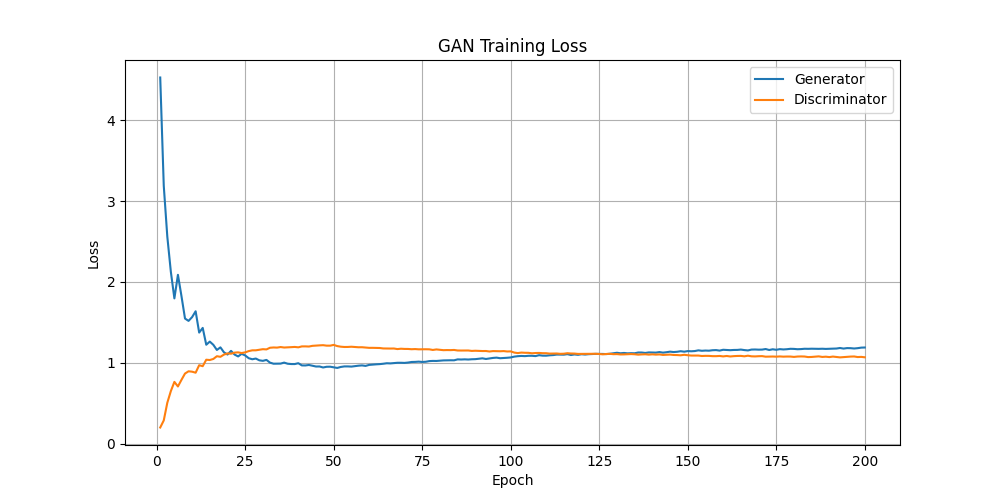
\includegraphics[width=\textwidth]{/Users/slkgaw/Proj/GANS/Logs/loss_gan/gan_loss_curve.png}
    \caption{GAN损失曲线}
\end{figure}
\clearpage
\begin{figure}[htbp]
    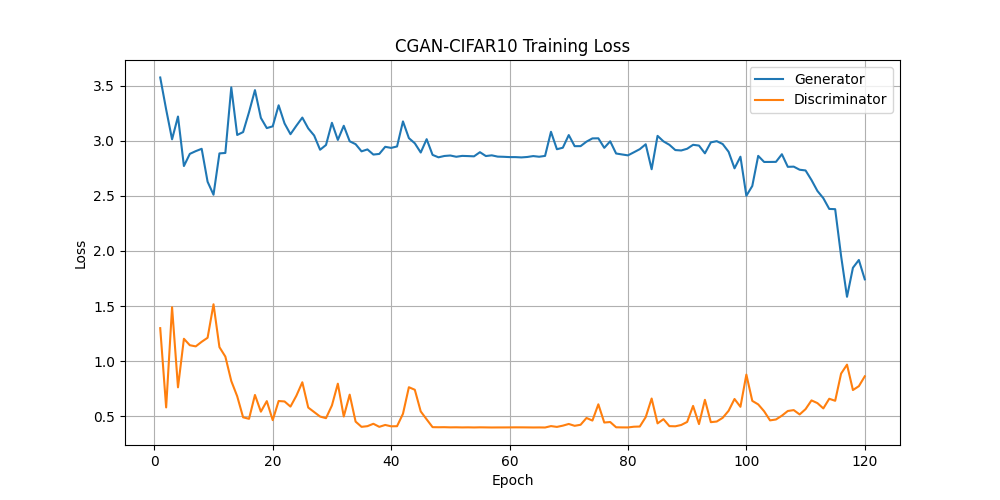
\includegraphics[width=\textwidth]{/Users/slkgaw/Proj/GANS/Logs/loss_cgan/cgan_loss_curve.png}
    \caption{CGAN损失曲线}
\end{figure}

从生成的图片来分析,可以发现 在多epoch + 小学习率 + 学习率schedule的训练策略下,GAN和CGAN生成图片的结果基本符合预期,
并且都展示了不错的多样性。
值得探讨的一点是,在模型大小,训练策略差不多的情况下CGAN的效果会比GAN的效果稍微好一些,具体体现在数字的
笔画更清晰,噪点更少。
这也正是CGAN的意义所在,C带标conditional,CGAN不仅是支持按类别生成,更重要的是类别能够知道模型进行训练
并知道模型生成。可以类比于Improved DDPM中使用的classifier guidance,这里的conditional相当于是一个ligth版本的
cls guidance。GAN的图片有不少噪点的原因,很大一部分程度是由于确实类别指导,在生成图像过程中有些拖泥带水,会附带小部分
其他类别的杂糅信息。

从损失曲线来看,GAN和CGAN基本都在30个epoch就在mnist数据集上达到了比较不错的效果。
值得探讨的是生成器和判别器的博弈关系,二者的loss曲线震荡的方向基本相反,符合“对抗”训练的过程。
而且因为有了类别指导,CGAN的收敛方向更准确,收敛速度更快。另一个可以探讨的点是,尽管在中后期生成器的损失有所上升,判别器的损失下降,
但是生成的图片的质量依然还在有上升的趋势,这也正是GAN的核心思想之一:纳什均衡。判别器的损失下降,表示判别器学到了更好的特征,有了更
严格的判定。因此促使生成器进一步提升。

\vspace{1cm}
完整的生成图片的样本随epoch的变化在附录


\clearpage
\subsubsection{WGAN和WGAN-GP}

\subsection{实验结果与分析}

\begin{figure}[htbp]
    \centering
    \begin{minipage}[t]{0.45\textwidth}
        \centering
        \includegraphics[width=\textwidth]{/Users/slkgaw/Proj/GANS/visual/WGAN/Wgan_sample_epoch_200.png}
        \caption{WGAN在200轮训练后的生成效果}
    \end{minipage}
    \hspace{0.04\textwidth}
    \begin{minipage}[t]{0.45\textwidth}
        \centering
        \includegraphics[width=\textwidth]{/Users/slkgaw/Proj/GANS/visual/WGAN-GP/wgan_gp_sample_epoch_200.png}
        \caption{WGAN-GP在200轮训练后的生成效果}
    \end{minipage}
\end{figure}

\vspace{1cm}

\begin{figure}[htbp]
    \centering
    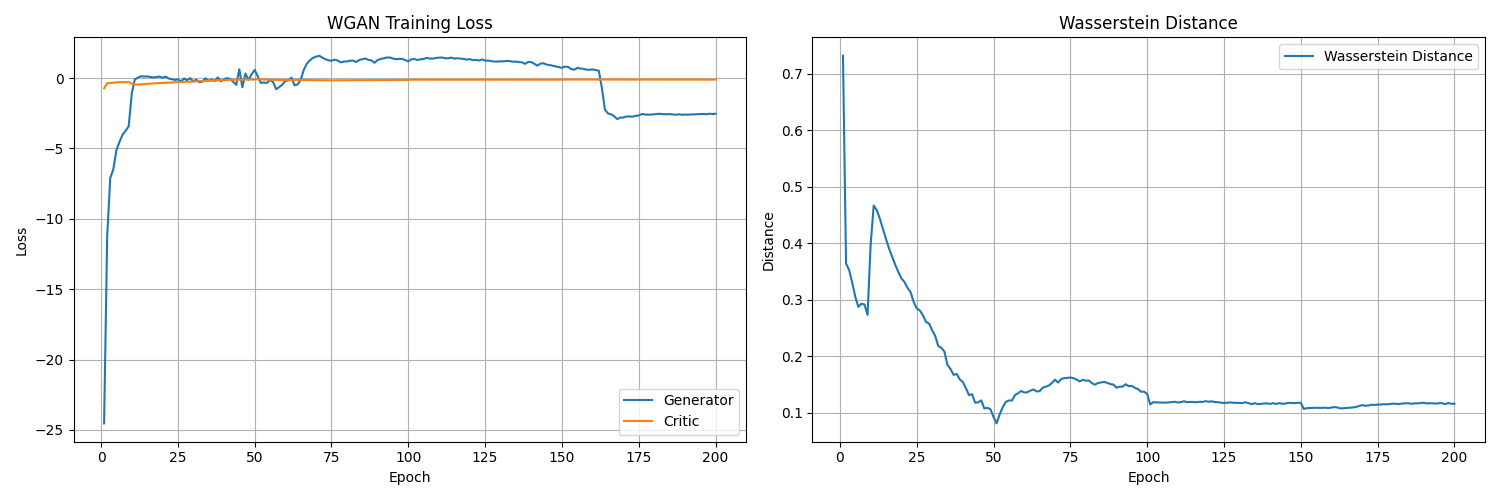
\includegraphics[width=\textwidth]{/Users/slkgaw/Proj/GANS/Logs/loss_wgan/wgan_loss_curve.png}
    \caption{WGAN损失曲线}
\end{figure}
\clearpage
\begin{figure}[htbp]
    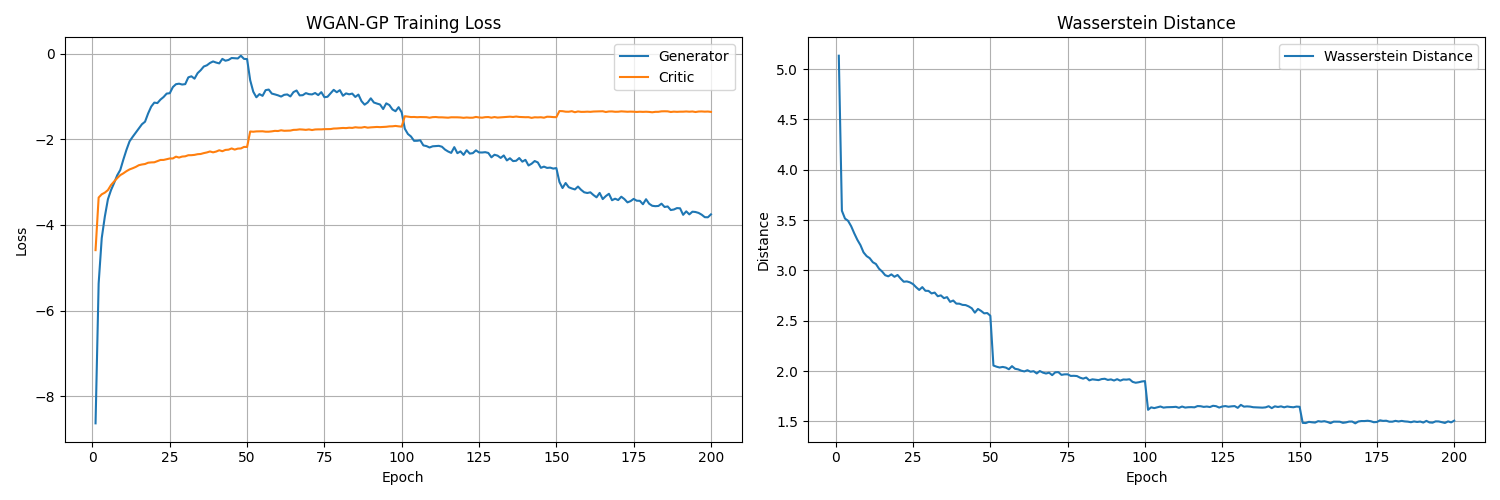
\includegraphics[width=\textwidth]{/Users/slkgaw/Proj/GANS/Logs/loss_wgan_gp/wgan_gp_loss_curve.png}
    \caption{WGAN-GP损失曲线}
\end{figure}

从生成的图片来分析,WGAN并没有达到预期的效果,尽管架构相比较普通的GAN有了明显的改进,但最终的效果却
不如朴素的GAN模型。在视觉效果上,WGAN生成的图片基本可以识别数字的种类,但是明显不够清晰,且有较多噪点。
而WGAN-GP在保留了WGAN所有相同的设定的情况下,仅引入了梯度惩罚,就能解决上述问题。

而从损失曲线和wasserstein距离曲线不难看出,GP版本使得训练相当稳定。而且每50个epoch就有一轮大幅的长进,
也恰恰对应了我预先设置的学习率schedule,使得模型在一个阶段学习得差不多后,能够在下个阶段学习更深层次的
特征细节。

以下将从几个角度分析WGAN最终效果差的原因已经GP能够显著改进的原因。

权重裁剪的设置,本实验采用了WGAN原论文的权重裁剪(clip\_value=0.01),但权重裁剪会导致Critic的表达能力受限,容易出现梯度消失或模型容量不足,进而影响生成器的训练效果。

网络结构较为简单,Generator和Critic均为全连接网络,且层数较少,模型容量有限,难以捕捉复杂的数据分布。对于图像生成任务,卷积结构通常更适合,能更好地提取空间特征。

优化器选择与超参数,WGAN原论文使用RMSprop优化器,但本实验中使用Adam也许不适配模型架构。此外,学习率设置过于复杂但是模型过于简单也有可能降低学习效率。

GP的作用在于让判别器的输出更加平滑,不会受到噪声已经误差的影响而突然跳变。
从曲线中不难看出,普通的WGAN曲线在初期十分陡峭且随后波动异常,大概是出现了数值不稳定的情况,进而影响了后续训练,使得效果大打折扣。
打个比方,如果把判别器想象成一条“评分曲线”,原始WGAN用“权重裁剪”让这条曲线变得很“平”,但这样容易让判别器变“笨”,分不清好坏。
而GP就像是在曲线上加了一个“弹簧”,让它既不会太陡峭(防止梯度爆炸),也不会太平(保留判别能力),始终保持适度的弹性。这样生成器和判别器就能更好地互相学习,生成效果也会更好。


\vspace{1cm}
完整的生成图片的样本随epoch的变化在附录


\newpage
\section{任务三:分析GAN在复杂数据集上的性能与模式坍塌问题}
\subsection{实验设置与方法}
任务三采用了BigGAN模型,BigGAN是google的Deepmind团队在2019年的一篇工作,是当时GAN系列的sota,在FID和IS两个指标上碾压当时所有的方法,
同时也证明了GAN具有很强的scale性能和较高的上限。

本实验在 ImageNet-1k 和 cifar10 等 数据集上做预训练,并在Animal-Faces上进行微调,且训练了多个版本的BigGAN,包括普通的BigGAN和conditional-BigGAN,已经不同图片size的版本,有128x128的版本也有512x512的版本。
模型参数由100M到1.5B不等

实验设备为4张 Nvidia 4090 24G GPU。

此外,本实验探究了大参数量的模型在复杂数据下的模式崩溃问题,以及探究了如何使用截断技巧来均衡样本的质量和多样性。

在接下来几个section将花大量篇幅分析模型架构,训练trick和结果分析。

\newpage
\subsection{模型架构}

以下为BigGAN用到的核心模块(以128x128的conditional-BigGAN为例):
\begin{itemize}
    \item 卷积层--conv2d,包括1x1的维度变换卷积和3x3的特征提取卷积
    \item 池化层--Pooling Layers,包括平均池化和全局平均池化和
    \item 激活函数--Activation Functions,包括relu,tanh和softmax
    \item 谱归一化--Spectral Normalization
    \item 批量归一化--Batch Normalization
    \item 条件嵌入层--Embedding Layers,包括条件BatchNorm的gamma/beta嵌入和投影判别器的类别嵌入
    \item 线性层--Linear Layers
    \item 自注意力模块--Self Attention
    \item 残差块--Residual Blocks
    \item 上采样层--Interpolation Layer 
    \item 分层噪声注入,将噪声z分割成多个块,在不同分辨率层注入不同的噪声块
\end{itemize}

以下是模型的架构总结(以128x128的conditional-BigGAN为例):
\vspace{1cm}


生成器路径:

z → Linear → 4×4 → Block1(8×8) → Block2(16×16) 
           → Block3(32×32,Attention) → Block4(64×64,Attention) 
           → Block5(128×128) → BatchNorm → ReLU → Conv → Tanh


\vspace{1cm}
判别器路径:

128×128 → Block1(64×64) → Block2(32×32,Attention) 
           → Block3(16×16,Attention) → Block4(8×8) → Block5(4×4) 
           → GlobalPool → Linear + Projection

\newpage

\begin{center}
\textbf{谱归一化:}
\end{center}

对权重矩阵 W,谱归一化将其约束为:
$$W_{SN} = \frac{W}{\sigma(W)}$$

其中 $\sigma(W)$ 是 W 的最大奇异值(谱范数)。

\vspace{0.5cm}

\textbf{作用:}
主要是为了防止深层次的大参数模型在训练过程中的数值不稳定问题,如梯度爆炸和梯度消失。
除此之外,谱归一化可以约束判别器的Lipschitz常数,稳定训练。
在本实验设置中,谱归一化应用于所有的卷积层、自注意力层和线性层,用于保持网络的表达能力。


\vspace{1cm}

\begin{center}
    \textbf{标量归一化:}
\end{center}
$$BN(x) = \gamma \frac{x - \mu}{\sqrt{\sigma^2 + \epsilon}} + \beta$$

\textbf{作用:}
批量归一化的本意是想加速训练速度,从数学角度解释BatchNorm可以缓解内部协变量偏移。
但更直观一点的说法是,一个batch内不同的通道的分布的均值方差不尽相同,使得每轮训练都
会因为这种分布的偏移而抖动震荡。
因此BatchNorm通过学习均值方差的约束来把各个通道的分布尽可能限制在差不多的position来稳定训练。
因为用了BatchNorm,对于学习率的选择可以更大胆一点,因为BatchNorm可以限制降低
模型对于学习率的敏感度同时减少对权重初始化的依赖。

\vspace{1cm}

\begin{center}
    \textbf{条件批标准化:}
\end{center}
给定类别标签 $y$,条件BatchNorm计算:
$$CBN(x, y) = \gamma(y) \frac{x - \mu}{\sqrt{\sigma^2 + \epsilon}} + \beta(y)$$

其中:
\begin{itemize}
    \item $\gamma(y) = Embedding_{\gamma}(y)$ - 类别特定的缩放因子
    \item $\beta(y) = Embedding_{\beta}(y)$ - 类别特定的偏移因子
    \item 每个类别都有独立的归一化参数
\end{itemize}

\textbf{作用:}
将类别信息直接注入到特征变换中,可以允许不同类别使用不同的特征分布。
这样在保证条件生成的质量和类别一致性的同时,也并没有比简单拼接复杂多少。



\begin{center}
    \textbf{自注意力模块:}
    \begin{align}
        Q &= Conv_{1 \times 1}(X) \quad \text{(Query)} \\    
        K &= Conv_{1 \times 1}(X) \quad \text{(Key)} \\
        V &= Conv_{1 \times 1}(X) \quad \text{(Value)} \\
        Attention &= Softmax(\frac{QK^T}{\sqrt{d_k}}) \\
        Output &= \gamma \cdot Conv_{1 \times 1}(V \cdot Attention) + X
    \end{align}
\end{center}

其中 $\gamma$ 是可学习参数,初始化为0。


\textbf{作用:}
自注意力能够捕获长距离空间依赖关系,相比卷积有更短最远距离。
在本实验模型架构中,自注意力模块选择在32x32和64x64这两个分辨率添加,平衡计算效率和结果。
自注意力的添加,能够显著提升生成图像的全局一致性,特别适合生成具有
复杂空间结构的图像。

\vspace{1cm}

\begin{center}
    \textbf{残差连接:}
\end{center}

\textbf{生成器块结构:}
\begin{align}
h &= ReLU(CBN(x, y)) \\
h &= Upsample(h) \quad \text{(最近邻上采样)} \\
h &= Conv_1(h) \\
h &= ReLU(CBN(h, y)) \\
h &= h + z_{chunk} \quad \text{(噪声注入)} \\
h &= Conv_2(h) \\
output &= h + Shortcut(Upsample(x))
\end{align}

\textbf{判别器块结构:}
\begin{align}
h &= ReLU(BN(x)) \quad \text{(预激活)} \\
h &= Conv_1(h) \\
h &= ReLU(BN(h)) \\
h &= Conv_2(h) \\
h &= AvgPool(h) \quad \text{(下采样)} \\
output &= h + Shortcut(AvgPool(x))
\end{align}

\textbf{作用:}
大幅解决梯度消失问题,支持更深网络的训练,
跳跃连接保持信息流动,预激活设计提升训练稳定性,允许网络学习恒等映射的微调。



\begin{center}
\textbf{最近邻上采样:}
\end{center}
$$Upsample(x) = Interpolate(x, scale\_factor=2, mode='nearest')$$

\textbf{作用:}
逐步将4×4特征图上采样到128×128。
最近邻插值可以避免引入伪影,且相比转置卷积更稳定,减少棋盘效应。
具体的上采样路径为:4×4 → 8×8 → 16×16 → 32×32 → 64×64 → 128×128

使用这种采样方案可以在不引入额外的可学习参数的前提下大幅提高计算效率,
且能避免转置卷积的不均匀覆盖问题并与后续卷积层配合生成高质量图像

\vspace{1cm}

\begin{center}
    \textbf{分层噪声注入}
\end{center}

\textbf{噪声分割策略:}
将输入噪声 $z \in \mathbb{R}^{128}$ 分割为5个块:
$$z = [z_0, z_1, z_2, z_3, z_4]$$
其中各块大小为 $[26, 26, 26, 25, 25]$

\textbf{注入位置:}
\begin{itemize}
    \item $z_0$:与类别嵌入拼接,输入初始线性层
    \item $z_1$:注入第1个生成器块 (4×4 → 8×8)
    \item $z_2$:注入第2个生成器块 (8×8 → 16×16)
    \item $z_3$:注入第3个生成器块 (16×16 → 32×32)
    \item $z_4$:注入第4个生成器块 (32×32 → 64×64)
\end{itemize}

\textbf{注入方式:}
$$h_{new} = h + Linear(z_{chunk}).unsqueeze(-1).unsqueeze(-1)$$

\textbf{作用:}
使得不同分辨率层获得独立的随机性输入,可以对粗粒度特征(低分辨率)和细粒度特征(高分辨率)分别控制。
此外从结果上分层注入噪声可以提升生成样本的多样性和质量,避免所有层共享单一噪声源的dominate现象,实现更精细的生成控制。

\newpage




\subsection{训练细节与训练技巧}

\subsubsection{学习率schedule}
原论文中采取恒定学习率+超大batch的方案,设备为8块google tpu v3,由于本实验的硬件限制,只能换用较小的batch加多epoch的方案。
而多epoch的训练最怕的就是训练中途抖动,累积误差影响最终结果。所以在本实验中采用了比较保守的学习率策略--余弦退火+warmup。
在训练初期学习率从0线性增加到初始学习率,持续到warmup\_steps步,避免初期训练梯度不稳定。
而在warmup后,学习率会按照余弦函数缓慢下降,最终趋于0。

关于学习率选择的一个解释是:因为128x128或512x512的图片非常占显存,因此batch选用很小。但是ImageNet数据集本身的多样性还是不错的。
所以在batch比较小的情况下,噪声和随机性的影响比例会比较大,如果此时保持和原论文中的学习率设置,那么会放大累积误差。
因此采用如此保守的学习率策略。

\vspace{0.5cm}
\noindent\textbf{schedule函数实现:}
\begin{lstlisting}[language=Python]
# 1. 定义 schedule 函数
def get_biggan_lr_lambda(warmup_steps, total_steps):
    def lr_lambda(step):
        if step < warmup_steps:
            return step / float(warmup_steps)
        else:
            progress = (step - warmup_steps) / float(max(1, total_steps - warmup_steps))
            return 0.5 * (1.0 + np.cos(np.pi * progress))
    return lr_lambda
\end{lstlisting}
\vspace{0.5cm}
\noindent\textbf{训练中的伪代码如下:}
\begin{lstlisting}[language=Python]
# 2. 初始化 scheduler
lr_lambda_func = get_biggan_lr_lambda(warmup_steps, total_steps)
scheduler_g = LambdaLR(optimizer_g, lr_lambda_func)
scheduler_d = LambdaLR(optimizer_d, lr_lambda_func)

# 3. 在训练循环中每步调用 step() 更新学习率
for epoch in range(num_epochs):
    for i, (images, labels) in enumerate(dataloader):
        # ...训练判别器和生成器...
        scheduler_g.step()
        scheduler_d.step()
        # ...其余训练代码...
# ...剩余代码...
\end{lstlisting}

\subsubsection{Hinge Loss}
在BigGAN原论文中使用了Hinge Loss这一损失函数,具体定义如下:
\begin{itemize}
    \item 对于判别器,Hinge Loss 旨在让真实样本的输出大于1,生成样本的输出小于-1,从而拉开两者的分界。
    \item 对于生成器,Hinge Loss 目标是最大化判别器对生成样本的输出(即让判别器认为生成样本更“真实”)。
\end{itemize}

实验表明,Hinge loss 这种损失函数能让GAN训练更稳定、生成效果更好,主要有以下几点原因:
1. 对判别器输出的限制更明确 2. 梯度更平滑,训练更稳定 3.让生成器有更明确的目标 4.降低梯度消失风险


\noindent\textbf{Hinge\_Loss代码实现如下:}
\begin{lstlisting}[language=Python]
def hinge_g_loss(fake_scores):
    # 生成器的 Hinge Loss
    # 目标:最大化 D(G(z)),等价于最小化 -D(G(z))
    return -torch.mean(fake_scores)

def hinge_d_loss(real_scores, fake_scores):
    # 判别器的 Hinge Loss
    # 损失形式:max(0, 1-D(real)) + max(0, 1+D(fake))
    real_loss = torch.mean(F.relu(1.0 - real_scores))
    fake_loss = torch.mean(F.relu(1.0 + fake_scores))
    return real_loss + fake_loss
\end{lstlisting}
\vspace{0.5cm}
\noindent\textbf{训练中的伪代码如下:}
\begin{lstlisting}[language=Python]
for epoch in range(num_epochs):
    for i, (images, labels) in enumerate(dataloader):
        # 判别器训练
        real_scores = D(x_real, y)
        fake_scores = D(G(z, y), y).detach()
        d_loss = mean(max(0, 1 - real_scores)) + mean(max(0, 1 + fake_scores))
        d_loss.backward()
        optimizer_d.step()

        # 生成器训练
        fake_scores = D(G(z, y), y)
        g_loss = -mean(fake_scores)
        g_loss.backward()
        optimizer_g.step()
\end{lstlisting}  

\subsubsection{正交正则化}
正交正则化是一种对权重矩阵施加约束的方法,目的是让权重矩阵的不同列
之间尽可能保持正交(即内积接近0)。这样做可以避免特征冗余,提高网络的表达能力和稳定性。
而原论文中则使用了改进版本(下方第二个版本),本实验未使用。公式如下:
$$ \mathcal{L}{ortho} = \beta \sum{l} \left| W_l^\top W_l - I \right|_F^2 $$
$$ R_\beta(W) = \beta \left| W^\top W \odot (1 - I) \right|_F^2 $$
\begin{itemize}
    \item $W_l$ 表示第 $l$ 层的权重矩阵(通常为全连接或卷积层的权重,展平成二维矩阵)
    \item $I$ 是单位矩阵,\odot 表示阿达马积
    \item $|\cdot|_F$ 表示Frobenius范数
    \item $\beta$ 是正交正则化的权重系数
\end{itemize}

\noindent\textbf{正交正则化代码实现如下:}
\begin{lstlisting}[language=Python]
def orthogonal_regularization(model, beta=1e-4):
    ortho_loss = 0.0
    for name, param in model.named_parameters():
        if 'weight' in name and param.dim() == 2:
            # param的形状是 (out_features, in_features)
            W = param
            WT_W = torch.matmul(W.t(), W)
            I = torch.eye(WT_W.size(0), device=W.device, dtype=W.dtype)
            ortho_loss += ((WT_W - I)**2).sum()
    return beta * ortho_loss

for epoch in range(num_epochs):
    for i, (images, labels) in enumerate(dataloader):
        # 判别器训练
        d_loss_ortho = orthogonal_regularization(discriminator)
        d_loss_total = d_loss_hinge + d_loss_ortho

        # 其他代码

        # 生成器训练
        g_loss_ortho = orthogonal_regularization(generator)
        g_loss_total = g_loss_hinge + g_loss_ortho
        # 其他代码
\end{lstlisting}  


\subsubsection{参数平均}
EMA(Exponential Moving Average,指数滑动平均)在GAN系列模型的训练中的主要作用是提升生成器的稳定性和生成质量。
具体的做法是先用初始的生成器状态来初始化EMA生成器,然后每个epoch训练结束后,用小权重系数将生成器的参数加权到
EMA生成器中,使得EMA生成器缓慢更新。

这种更新策略十分有助于减弱训练过程中的噪声和震荡,使参数变化更加平滑。
经实验证明,在训练后期,直接用EMA生成器生成的样本通常比普通生成器更清晰、更稳定,FID/IS等指标更好。

此外,EMA能缓解模型在训练后期的过拟合和模式崩溃问题,使生成器保持更好的泛化能力。
因此,评估时常用EMA生成器而非当前生成器,得到的分数更能反映模型的真实性能。

EMA的技巧要想达到好的效果的前提是EMA的alpha参数设置,设置过大容易导致学得太浅,学习不到生产图片的分布,
如果alpha设置过大,在训练后期就很有可能和普通生成器一样,甚至会过拟合数据。
因此实际的alpha选择需要根据模型规模和训练规模来决定。

\vspace{1cm}

\begin{lstlisting}[language=python]
# 初始化EMA生成器
ema_generator = copy(generator)

for each training step:
    # ...训练生成器和判别器...
    # EMA参数更新
    for ema_param, param in zip(ema_generator.parameters(), generator.parameters()):
        ema_param = alpha * ema_param + (1 - alpha) * param

for each evaluation:
    # 用普通生成器生成样本,计算指标
    samples = generator.generate(...)
    IS, FID = evaluate(samples)
    # 用EMA生成器生成样本,计算指标
    ema_samples = ema_generator.generate(...)
    EMA_IS, EMA_FID = evaluate(ema_samples)
\end{lstlisting}

\vspace{1cm}
在checkpoints保存到时候要把ema\_generator包括进去,同时保证ema\_generator保持eval模式,
避免计算梯度从而出现参数更新错误。

\subsubsection{多卡训练的策略trick}

为了加速训练,多卡训练在如今的深度学习中已经变得十分常见,且十分必要。从训练效果上来讲,多卡训练允许训练时候使用更大的batch,
而更大的batch能显著减少噪音和误差带来的干扰,尤其是在GAN这种训练敏感的模型上,能够有效稳定训练过程。

为了模仿原论文中的超大batch,有一个小trick是累积梯度法,即每step步做一次反向,其余时刻只累积梯度,优化器不做优化。
示例代码如下:
\begin{lstlisting}[language=python]
# 1. 构建模型
generator = Generator(...)
discriminator = Discriminator(...)

# 2. 多卡包装
if GPU数量 > 1:
    generator = DataParallel(generator)
    discriminator = DataParallel(discriminator)

# 3. 优化器和累计步数
optimizer_g = Adam(generator.parameters(), ...)
optimizer_d = Adam(discriminator.parameters(), ...)
accumulation_steps = 4  # 例如4个小batch等价于1个大batch

# 4. 训练循环
for epoch in range(num_epochs):
    optimizer_g.zero_grad()
    optimizer_d.zero_grad()
    for i, (images, labels) in enumerate(dataloader):
        # 判别器训练
        d_loss = compute_d_loss(real_scores, fake_scores) / accumulation_steps
        d_loss.backward()
        if (i + 1) % accumulation_steps == 0:
            optimizer_d.step()
            optimizer_d.zero_grad()

        # 生成器训练
        g_loss = compute_g_loss(fake_scores) / accumulation_steps
        g_loss.backward()
        if (i + 1) % accumulation_steps == 0:
            optimizer_g.step()
            optimizer_g.zero_grad()
\end{lstlisting}

\newpage
\subsection{实验结果与分析}
\subsubsection{样本分析}
总的来说本实验训练的BigGAN模型在ImageNet上预训练的效果比较好,但是在AnimalFaces上微调的效果不尽人意(在后面局限性那一节有提到)。
下图均为ImageNet的生成结果。以下图片类别分别为wolf,hamburger,truck,daisy,随机。
\vspace{1cm}


\begin{figure}[htbp]
    \centering
    \includegraphics[width=1.0\textwidth]{/Users/slkgaw/Proj/GANS/visual/BigGAN/128_by_class/19.jpg}
    \caption{按类别生成(wolf)}
\end{figure}

\begin{figure}[htbp]
    \centering
    \includegraphics[width=1.0\textwidth]{/Users/slkgaw/Proj/GANS/visual/BigGAN/128_by_class/34.jpg}
    \caption{按类别生成(hamburger)}
\end{figure}

\begin{figure}[htbp]
    \centering
    \includegraphics[width=1.0\textwidth]{/Users/slkgaw/Proj/GANS/visual/BigGAN/128_by_class/52.jpg}
    \caption{按类别生成(trunk)}
\end{figure}
\newpage
\begin{figure}[htbp]
    \centering
    \includegraphics[width=1.0\textwidth]{/Users/slkgaw/Proj/GANS/visual/BigGAN/128_by_class/53.jpg}
    \caption{按类别生成(daisy)}
\end{figure}


\foreach \i in {1} {
    \begin{figure}[htbp]
        \centering
        \includegraphics[width=1.0\textwidth]{/Users/slkgaw/Proj/GANS/visual/BigGAN/128_random/\i.jpg}
        \caption{随机生成}
    \end{figure}
}

\vspace{1cm}
从生成图片的效果上来看,BigGAN因为属于GAN系列模型,在生成质量这一方面十分强劲,在部分生成样本中保持了和数据集
接近的保真度。但与此同时,模型生成图片的多样性并不算好(在局限性小节会详细说明),就比如雏菊这个类别生成的样本基本都很相似。

\newpage

\subsubsection{Truncation Trick}
原论文中提及了一个十分有用的技巧,叫做truncation trick,即在生成随机高斯噪声时,限定噪声的空间范围,只允许高概率空间中的噪声用于图片生成。
这样能够大幅提高图标质量但同时也会大幅降低生成图片的多样性。以下展示不同截断值生成的图片效果。

\foreach \i in {0.2, 0.4, 0.6, 0.8, 1.0}{
    \begin{figure}[H]
        \centering
        \includegraphics[width=0.9\textwidth]{/Users/slkgaw/Proj/GANS/visual/BigGAN/truncation/trunc_\i/cat.jpg}
        \caption{trunc=\i}
    \end{figure}
    \par\vspace{0cm}
}


Truncation的伪代码如下:
\begin{lstlisting}[language=python]
# 采样高斯噪声
z = np.random.randn(batch_size, z_dim)
# 截断
truncation = 0.5
z_t = np.clip(z, mean - truncation * std, mean + truncation * std)
  
\end{lstlisting}

\subsubsection{插值分析}
判断GAN系列模型生成质量的一个做法是对给定的两组(z, c)对(z为噪声,c为类别),通过球面线性插值,来获得多组(z, c)对。
然后以此送入生成器进行生成,通过观察一系列样本的特征连续性来判断模型在拟合各个类别分布时的实际效果。

一般来说,对于相似的类别,比如同是动物,或者相似的类别语境,比如鸟和果实都在树上,特征变化应当表现的均匀,过度平滑,如此便可基本可以确定类别间分布在隐空间的同一个超球面上,如下图所示。

\vspace{0.5cm}

\foreach \i in {1,2,3,4,16,14,39}{
    \begin{figure}[H]
        \centering
        \includegraphics[width=0.9\textwidth]{/Users/slkgaw/Proj/GANS/visual/BigGAN/interpolation/\i.png}
    \end{figure}
}

\newpage

\subsubsection{局限性}

本实验尽管在ImageNet上表现良好,但是在微调的时候出现了严重的模式坍塌问题。无论在训练的什么阶段生成的图片基本只有1-2种相似模式,可以说基本是过拟合到
某一显著的图片模式上了。初步分析原因,数据集的差异是造成这一结果的主要因素。

AnimalFaces数据集(见附录)包含动物面部的512x512的图片,只有三个类,分别是cat,dog和wild,但是每个类的多样性非常好。
形象地说,一个类别的分布十分不好建模,比如狗🐶有非常多的品种,金毛犬,松狮,腊肠犬,长相都十分不一样。
而本实验预训练时所用的ImageNet对这种区别很大的不同品种的狗其实是算分为不同的类别。
\textbf{同时这也再一次证实了GAN系列模型的缺点,多样性不足,容易出现模式坍塌现象。
因此GAN模型不能像diffusion模型那样用text做细粒度的控制,而且GAN模型在语境细节很多的类别的情况下的生成效果非常差。
}
从微调曲线上亦可看出BigGAN模型在AnimalFaces数据集上训练十分不稳定,尽管用了很大batch,模型优化的方向依然飘摇不定,反复震荡。
微调结果和微调损失如下:

\begin{figure}[H]
    \centering
    \foreach \i in {1,3,2}{
        \begin{minipage}[t]{0.3\textwidth}
            \centering
            \includegraphics[width=\textwidth]{/Users/slkgaw/Proj/GANS/visual/BigGAN/cat/group3/sample_\i.png}
        \end{minipage}
    }
    \caption{微调后,模型基本只能生成这三张样貌的猫,而且相似度很高}
\end{figure}

\begin{figure}[H]
    \centering
    \includegraphics[width=0.8\textwidth]{/Users/slkgaw/Proj/GANS/visual/BigGAN/loss_curves.png}
    \caption{BigGAN在AnimalFaces数据集上微调的损失曲线}
\end{figure}

















\newpage
\section{附录}


% ===== GAN 结果展示 =====
\subsection{GAN不同epoch生成的样本}
\vspace{1.5cm}
\begin{figure}[htbp]
    \centering
    \foreach \i/\ep in {1/20,2/40,3/60,4/80,5/100,6/120,7/140,8/160,9/180,10/200} {
        \begin{minipage}[t]{0.23\textwidth}
            \centering
            \includegraphics[width=\textwidth]{/Users/slkgaw/Proj/GANS/visual/GAN/gan_sample_epoch_\ep.png}
            \caption*{GAN \ep~epoch}
        \end{minipage}
        \ifnum\i=4 \par\vspace{0.2cm}\fi
        \ifnum\i=8 \par\vspace{0.2cm}\fi
    }
    \caption{GAN不同epoch生成样本}
    \label{fig:gan_epochs}
\end{figure}


\newpage

% ===== CGAN 结果展示 =====
\subsection{CGAN不同epoch生成的样本}
\vspace{1.5cm}
\begin{figure}[htbp]
    \centering
    \foreach \i/\ep in {1/20,2/40,3/60,4/80,5/100,6/120,7/140,8/160,9/180,10/200} {
        \begin{minipage}[t]{0.23\textwidth}
            \centering
            \includegraphics[width=\textwidth]{/Users/slkgaw/Proj/GANS/visual/CGAN/cgan_sample_epoch_\ep.png}
            \caption*{CGAN \ep~epoch}
        \end{minipage}
        \ifnum\i=4 \par\vspace{0.2cm}\fi
        \ifnum\i=8 \par\vspace{0.2cm}\fi
    }
    \caption{CGAN不同epoch生成样本}
    \label{fig:cgan_epochs}
\end{figure}


\newpage
% ===== WGAN-GP 结果展示 =====
\subsection{WGAN-GP不同epoch生成的样本}
\vspace{1.5cm}
\begin{figure}[htbp]
    \centering
    \foreach \i/\ep in {1/20,2/40,3/60,4/80,5/100,6/120,7/140,8/160,9/180,10/200} {
        \begin{minipage}[t]{0.23\textwidth}
            \centering
            \includegraphics[width=\textwidth]{/Users/slkgaw/Proj/GANS/visual/WGAN-GP//wgan_gp_sample_epoch_\ep.png}
            \caption*{WGAN-GP \ep~epoch}
        \end{minipage}
        \ifnum\i=4 \par\vspace{0.2cm}\fi
        \ifnum\i=8 \par\vspace{0.2cm}\fi
    }
    \caption{WGAN-GP不同epoch生成样本}
    \label{fig:wgan_gp_epochs}
\end{figure}

\newpage
% ==== BigGAN 按类别随机样本 ====
\subsection{BigGAN按类别生成样本展示 128x128}
\begin{center}
\foreach \i in {1,...,7} {
    \includegraphics[width=0.8\textwidth]{/Users/slkgaw/Proj/GANS/visual/BigGAN/128_by_class/\i.jpg}
    \par\vspace{0.1cm}
}
\end{center}
% 每页7张图片,共9页
\foreach \page in {1,...,7} {
    \begin{figure}[htbp]
        \centering
        \foreach \i in {1,...,7} {
            \pgfmathtruncatemacro{\imgnum}{\page*7+\i}
            \ifnum\imgnum<57
                \includegraphics[width=0.8\textwidth]{/Users/slkgaw/Proj/GANS/visual/BigGAN/128_by_class/\imgnum.jpg}
                \par\vspace{0.2cm}
            \fi
        }
        \caption*{BigGAN按类别生成样本(第\the\numexpr\page+1\relax 页)}
    \end{figure}
}

\newpage

\subsection{BigGAN随机样本展示 128x128}
\vspace{1cm}
\begin{center}
\foreach \i in {1,...,3} {
    \includegraphics[width=0.8\textwidth]{/Users/slkgaw/Proj/GANS/visual/BigGAN/128_random/\i.jpg}
    \par\vspace{0.2cm}
}
\end{center}

\foreach \page in {1,...,2} {
    \begin{figure}[htbp]
        \centering
        \foreach \i in {1,...,3} {
            \pgfmathtruncatemacro{\imgnum}{\page*3+\i}
            \ifnum\imgnum<10
                \includegraphics[width=0.8\textwidth]{/Users/slkgaw/Proj/GANS/visual/BigGAN/128_random/\imgnum.jpg}
                \par\vspace{0.2cm}
            \fi
        }
        \caption*{BigGAN随机样本展示(第\the\numexpr\page+1\relax 页)}
    \end{figure}
}

\subsection{BigGAN随机样本展示 512x512}
\vspace{1cm}
\begin{center}
\foreach \i in {1,...,3} {
    \includegraphics[width=0.8\textwidth]{/Users/slkgaw/Proj/GANS/visual/BigGAN/512_random/\i.jpg}
    \par\vspace{0.2cm}
}
\end{center}

\foreach \page in {1} {
    \begin{figure}[htbp]
        \centering
        \foreach \i in {1,...,3} {
            \pgfmathtruncatemacro{\imgnum}{\page*3+\i}
            \ifnum\imgnum<6
                \includegraphics[width=0.8\textwidth]{/Users/slkgaw/Proj/GANS/visual/BigGAN/512_random/\imgnum.jpg}
                \par\vspace{1cm}
            \fi
        }
        \caption*{BigGAN随机样本展示(第\the\numexpr\page+1\relax 页)}
    \end{figure}
}


\subsection{BigGAN不同类别间插值采样}
\vspace{1cm}
\begin{center}
\foreach \i in {1,...,8} {
    \includegraphics[width=0.8\textwidth]{/Users/slkgaw/Proj/GANS/visual/BigGAN/interpolation/\i.png}
    \par\vspace{1cm}
}
\end{center}
\foreach \page in {1,2,3,4} {
    \begin{figure}[htbp]
        \centering
        \foreach \i in {1,...,8} {
            \pgfmathtruncatemacro{\imgnum}{\page*3+\i}
            \ifnum\imgnum<41
                \includegraphics[width=0.8\textwidth]{/Users/slkgaw/Proj/GANS/visual/BigGAN/interpolation/\imgnum.png}
                \par\vspace{1cm}
            \fi
        }
        \caption*{BigGAN不同类别间插值展示(第\the\numexpr\page+1\relax 页)}
    \end{figure}
}

\newpage
\subsection{AninmalFaces数据集展示}
\begin{figure}[H]
    \centering
    \includegraphics[width=1.0\textwidth]{/Users/slkgaw/Proj/GANS/BigGAN/batch_sample.png}
\end{figure}
\begin{figure}[H]
    \centering
    \includegraphics[width=1.0\textwidth]{/Users/slkgaw/Proj/GANS/visual/BigGAN/batch_sample.png}
\end{figure}
\end{document}

